\chapter{Star Contraction}
\label{ch:graphcon::star}

\begin{preamble}
This chapter covers star partition and star contraction, an
efficient and parallel 
%
\href{def:graphcon::intro::graphcon::technique}{graph-contraction technique}
%
for general graphs. 
\end{preamble}

\section{Star Partition}
\label{sec:graphcon::star::partition}


In an 
%
\href{sec:graphcon::edge::partition}{edge partition},
%
if an edge incident on a vertex~$v$ is selected
as a block, then none of the other edges incident on $v$ can be their
own block.
%
This limits the effectiveness of the edge partition technique, because
it is unable to contract graphs with high-degree vertices
significantly.
%
In this section, we describe an alternative technique, star partition, that does not have this limitation.

\begin{flex}
\begin{definition}[Star Partition]
\label{def::graphcon::star-partition}
A~\defn{star partition} of a graph $G$ is a partition of $G$ where each block
is vertex-induced subgraph with respect to a 
%
\href{def:graphcon::edge::analysis::star::star-graph}{star graph}.
\end{definition}

\begin{example}
\label{ex:graphcon::star::partition::1}
Consider star graph with center $v$ and eight satellites.
  \begin{center}
  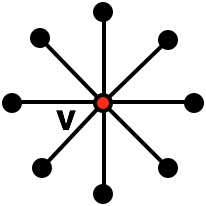
\includegraphics[width=1.5in]{./graph-contraction/media-star/star-graph1.jpg}
  \end{center}

\begin{itemize}
\item A partition consisting of the whole graph is a star partition, where 
the only block is the graph itself, induced by the star graph.

\item A partition where each block is an isolated vertex is a star
  partition, because each block is a vertex-induced subgraph of a
  single vertex, which is a star.
\end{itemize}

\end{example}


\begin{example}
\label{ex:graphcon::star::partition::2}


Consider the graph shown below on the left.
%
To partition this graph, we first find two disjoint stars, which are
highlighted.
%
Each star induces a block consisting of its vertices and the
corresponding edges of the graph.
%
These two blocks form a star partition the graph.
%
%% TODO: Comment this out in favor of the important block below.
Note that in a star partition, a block might not be a star.
\begin{center}
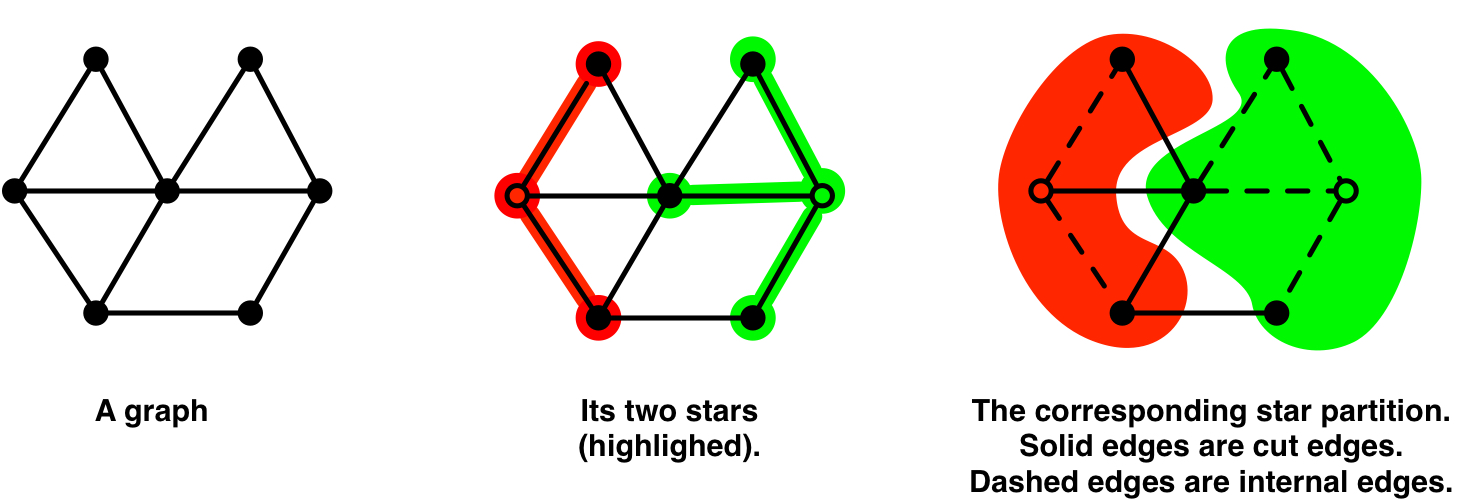
\includegraphics[width=0.9\textwidth]{./graph-contraction/media-star/star-decomposition-1.jpg}
\end{center}
\end{example}
\end{flex}

%% \begin{important}
%% In a star partition, a partition might not be a star.
%% \end{important}
%% \begin{teachask}
%% How can we star-partition a graph? 
%% \end{teachask} 

\begin{gram}[Constructing a Star Partition (Sequential)]
\label{graphcon::star::partition::seq}

We can construct a star partition sequentially by iteratively adding
stars until the vertices are exhausted as follows.

\begin{itemize}

\item Select an arbitrary vertex $v$ from the graph and make $v$ the
  center of a star.

\item Attach as satellites all the neighbors of $v$ in the graph.

\item Remove $v$ and its satellites from the graph.

\end{itemize}
%
\end{gram}


\begin{note}
\label{graphcon::star::partition::implementing-heads}

Since most machines don't have true sources of randomness, in practice
the function $\cdvar{heads}$ is usually implemented with a
pseudorandom number generator or with a good hash function.

In the algorithm, Line~\linegcstarmerge{} creates a set of
singleton tables and merges them.
%
This can be implemented using sets and tables as follows.
%
\[
\begin{array}{ll}
  \cdvar{Set.reduce}
  & (\cdvar{Table.union}~(\cfn{(x,y)}{x}))
\\
& \emptyset
\\
& \cset{\cset{u \mapsto v} : (u,v) \in \mathit{TH}}
\end{array}
\]
Note that we supply to the $\cdvar{union}$ operation a function that selects the first of the two possibilities; this is an arbitrary choice and we could have favored the second.

\end{note}

\begin{example}
\label{ex:graphcon::star::partition::alg}

Consider the star partition illustrated below.
\begin{center}
  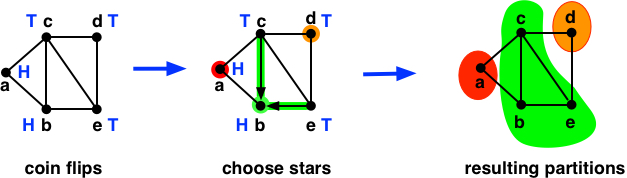
\includegraphics[width=6in]{./graph-contraction/media-star/star-find0.jpg}
\end{center}

The  star-partition algorithm proceeds on this example as follows.
%
First, it computes
%
\[
\mathit{TH} =
\cset{(\vname{c},\vname{a}),(\vname{c},\vname{b}),(\vname{e},\vname{b})},
\]
%
as the edges from satellites to centers.  
%
Now, it
converts each edge into a singleton table, and merges all the tables
into one
table, which is going to become a part of the partition map:
%
\[
P_s = \cset{\vname{c} \mapsto \vname{b},\vname{e} \mapsto \vname{b}}.
\]
%
Note that the edge $(\vname{c},\vname{a})$ has been removed since when
uniting the tables, we select only one element for each key in the
domain.  
%
Now for all remaining vertices
%
$V' = V \setminus \cdvar{domain}(P) = \cset{\vname{a},\vname{b},\vname{d}}$
we map them to themselves, giving:
%
\[
P_c = \cset{\vname{a} \mapsto \vname{a}, \vname{b} \mapsto \vname{b},
  \vname{d} \mapsto \vname{d}}.
\]
%
The vertices in $P'$ are the centers.
%
Finally we merge $P$ and $P'$ to obtain the partition map
%
\[
P_s \cup P_c = \cset{\vname{a} \mapsto \vname{a}, \vname{b} \mapsto \vname{b}, \vname{c} \mapsto \vname{b}, \vname{d} \mapsto
    \vname{d}, \vname{e} \mapsto \vname{b}}.
\]
\end{example}
\end{flex}


%% \begin{todo}
%% This theorem needs a proof.  What is the graph representation? 
%% It seems like it is an edge set representation.

%% The big union would require logn span do we need inject here?

%% \end{todo}


\section{Star Contraction}
\label{sec:graphcon::star::contract}

\begin{definition}[Star Contraction]
\label{def:graphcon::star-contraction}
\defn{Star contraction} is an instance of graph contraction that uses
star partitions to contract the graph.
\end{definition}


